\documentclass[12pt, titlepage]{article}

\usepackage{fullpage} %full page typesetting
\usepackage{setspace} %allows for non-singlespacing
\usepackage{graphicx} %graphics capabilities
\usepackage{latexsym} %extra symbols
\usepackage{rotating} %rotation for figures
\usepackage{longtable} %tables that fill more than a single page
%\usepackage{hyperref} %hypertext links in the document
\usepackage{natbib} %better bibliographies
\usepackage{authblk} %author and affiliation in opening
\usepackage{mathpazo} %use palatino font, rather than times
\usepackage{appendix}
\usepackage{lscape}
\usepackage{tabulary}
\usepackage[nottoc]{tocbibind}
\usepackage[colorlinks=true,linkcolor=blue,citecolor=cyan]{hyperref}
\usepackage{ifthen}
\usepackage{float}
\usepackage{subcaption}
\usepackage{mwe}
\usepackage{caption}


\title{\tb{Place of Residence and Political Attitudes in Democracies Worldwide \\ {\large Online Appendix A -- Box Plots} }}

\author{Jennifer Lin}
\affil{New College of Florida}

\newcommand\e{\emph}
\newcommand\tb{\textbf}
\newcommand\un{\underline}
\newcommand\txt{\texttt}

\doublespacing 

\begin{document}

\begin{singlespace}
\maketitle
\end{singlespace}

\section{Global Trends}
This Appendix features the box plots for each country divided by place of residence and by dependent variable. They show the location of the minimum, first quartile, median, third quartile and maximum scores for each place based on both self-placement ideology and the liberalism/issue stances dependent variable. The definitions for each place identifier coincides with the identifiers used in the CSES such that 

\begin{quote}
	1 = Rural Village \\
	2 = Small Town \\
	3 = Suburban City \\
	4 = Urban City 
\end{quote}

Each box-plot is labeled with a caption to identify the dependent variable that is used to create the data.

\begin{figure}[H]
	\centering
	\begin{subfigure}[b]{0.475\textwidth}   
		\centering 
		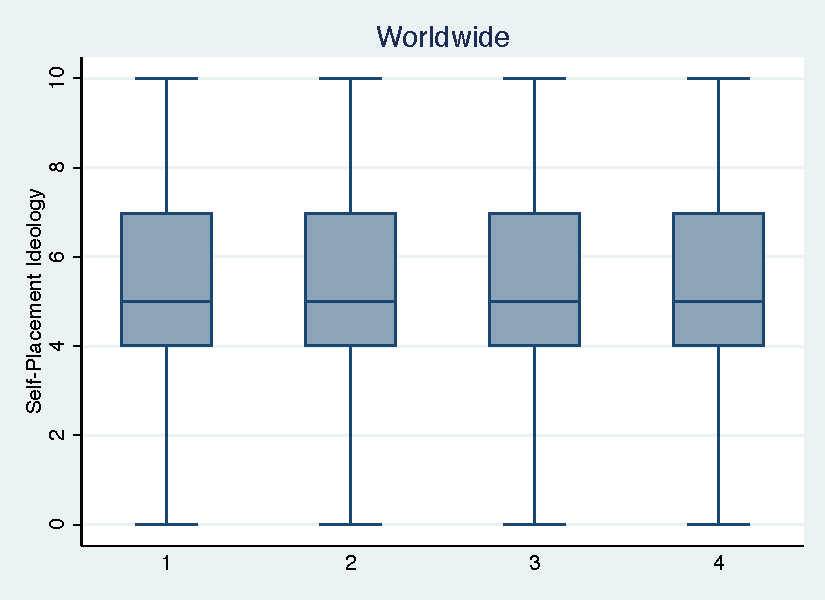
\includegraphics[width=\textwidth]{IdeoBP/BoxAllIdeo}
		\caption{Self-Placement Ideology}
	\end{subfigure}
	\hfill
	\begin{subfigure}[b]{0.475\textwidth}
		\centering 
		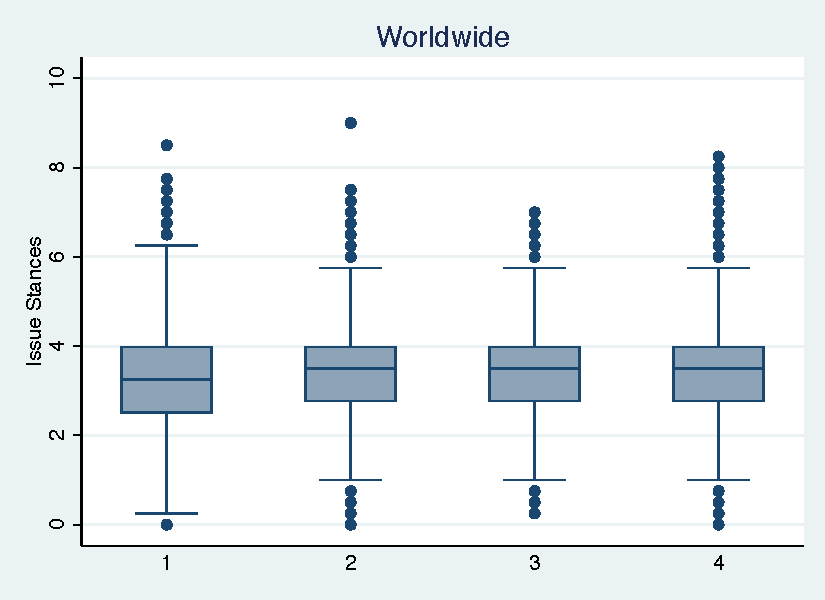
\includegraphics[width=\textwidth]{BoxLib/BoxAllLib}
		\caption{Issue Stances}
	\end{subfigure}
	\caption{Global Trends}
	\label{Worldwide}
\end{figure}

\section{Country Specific}

\begin{figure}[H]
	\centering
	\begin{subfigure}[b]{0.475\textwidth}   
	\centering 
	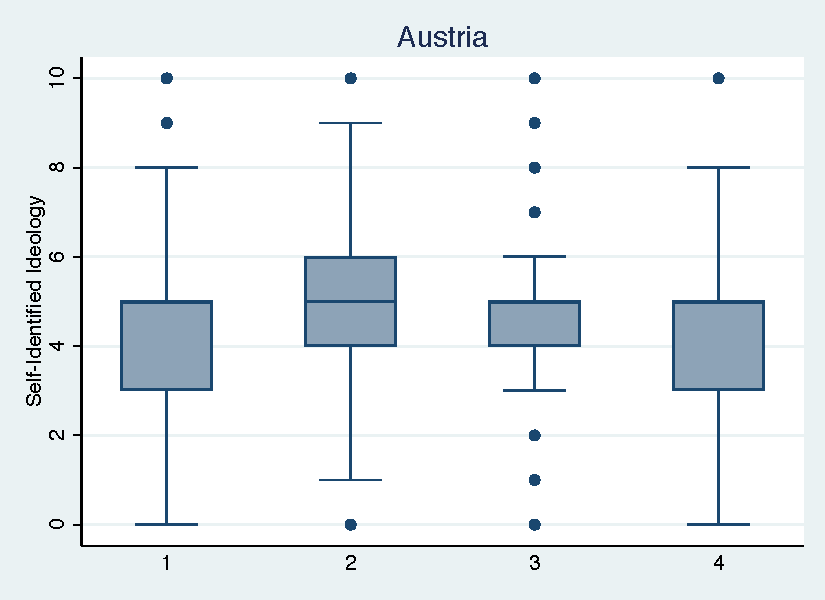
\includegraphics[width=\textwidth]{IdeoBP/Austria}
	\caption{Self-Placement Ideology}
	\end{subfigure}
	\hfill
	\begin{subfigure}[b]{0.475\textwidth}
	\centering 
	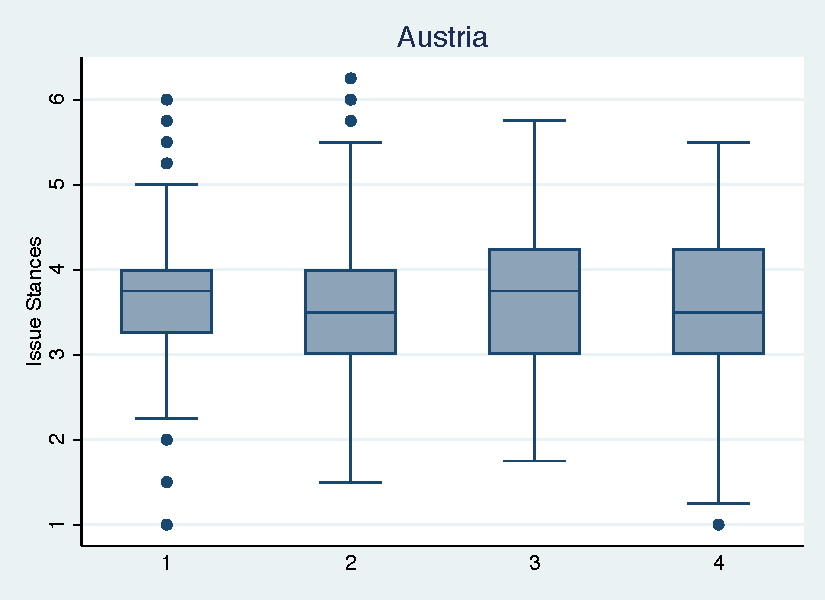
\includegraphics[width=\textwidth]{BoxLib/Austria}
	\caption{Issue Stances}
	\end{subfigure}
	\caption{Austria}
	\label{Austria}
\end{figure}

\begin{figure}[H]
	\centering
	\begin{subfigure}[b]{0.475\textwidth}   
		\centering 
		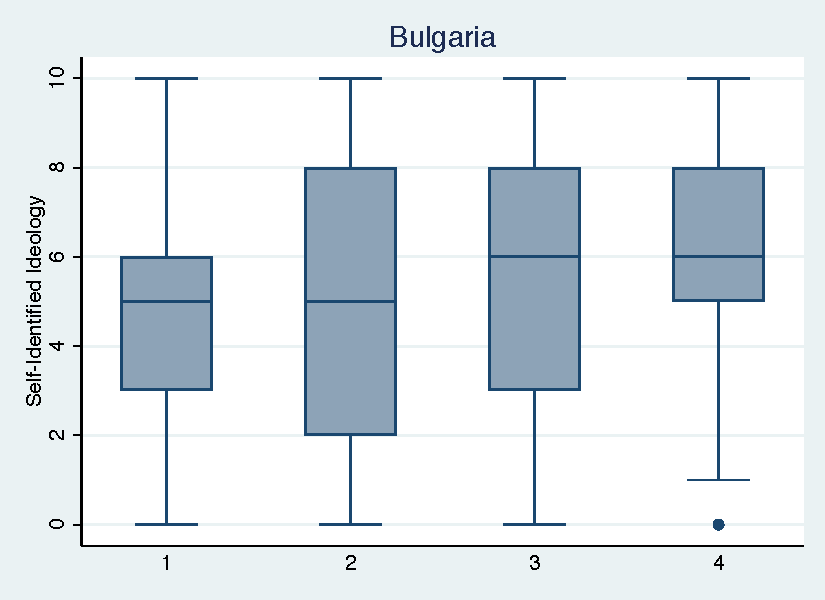
\includegraphics[width=\textwidth]{IdeoBP/Bulgaria}
		\caption{Self-Placement Ideology}
	\end{subfigure}
	\hfill
	\begin{subfigure}[b]{0.475\textwidth}
		\centering 
		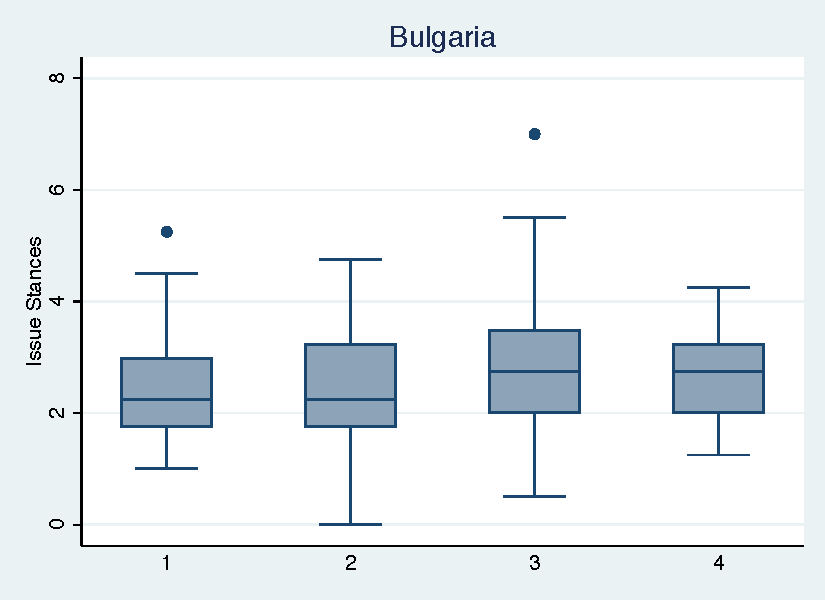
\includegraphics[width=\textwidth]{BoxLib/Bulgaria}
		\caption{Issue Stances}
	\end{subfigure}
	\caption{Bulgaria}
	\label{Bulgaria}
\end{figure}

\begin{figure}[H]
	\centering
	\begin{subfigure}[b]{0.475\textwidth}   
		\centering 
		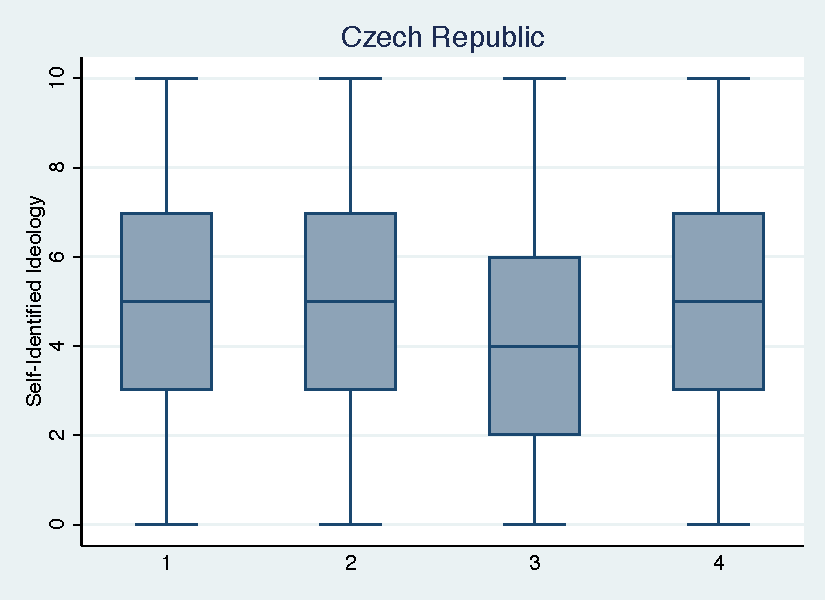
\includegraphics[width=\textwidth]{IdeoBP/Czech}
		\caption{Self-Placement Ideology}
	\end{subfigure}
	\hfill
	\begin{subfigure}[b]{0.475\textwidth}
		\centering 
		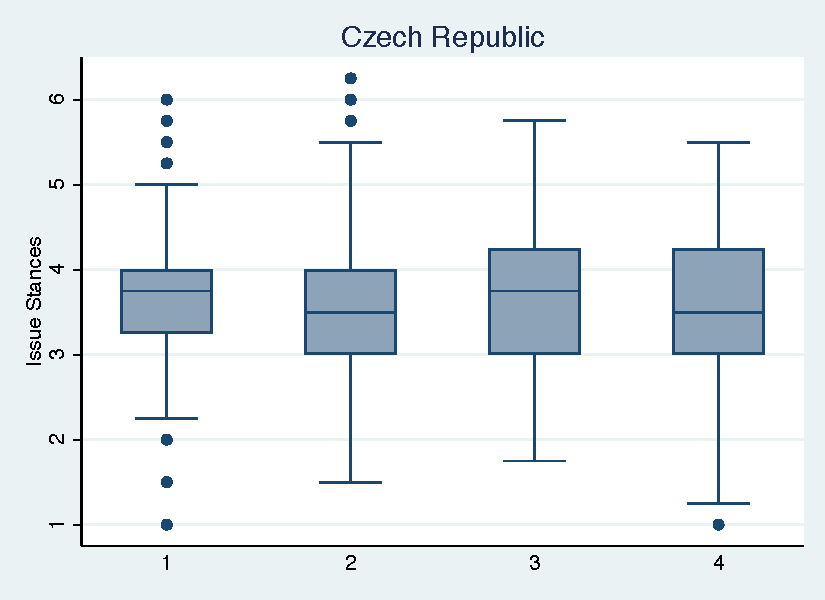
\includegraphics[width=\textwidth]{BoxLib/Czech}
		\caption{Issue Stances}
	\end{subfigure}
	\caption{Czech Republic}
	\label{Czech}
\end{figure}

\begin{figure}[H]
	\centering
	\begin{subfigure}[b]{0.475\textwidth}   
		\centering 
		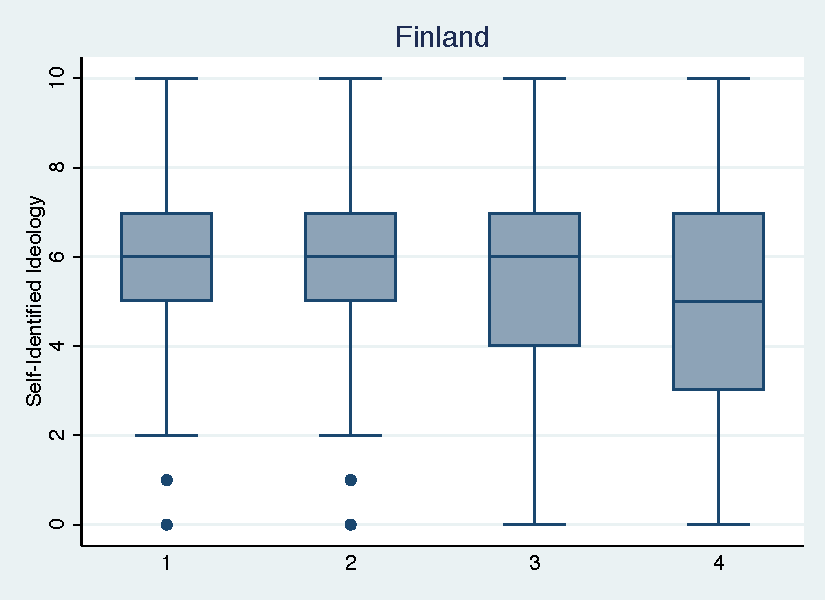
\includegraphics[width=\textwidth]{IdeoBP/Finland}
		\caption{Self-Placement Ideology}
	\end{subfigure}
	\hfill
	\begin{subfigure}[b]{0.475\textwidth}
		\centering 
		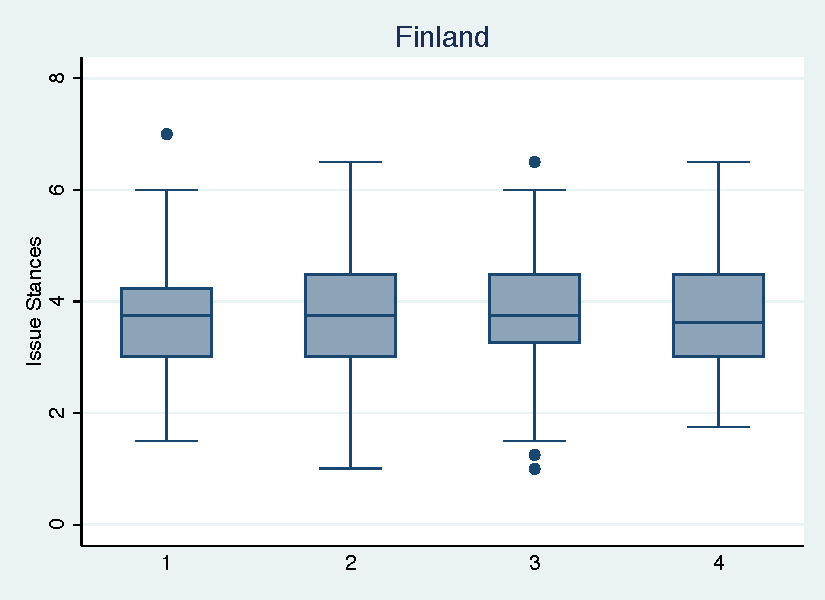
\includegraphics[width=\textwidth]{BoxLib/Finland}
		\caption{Issue Stances}
	\end{subfigure}
	\caption{Finland}
	\label{Finland}
\end{figure}

\begin{figure}[H]
	\centering
	\begin{subfigure}[b]{0.475\textwidth}   
		\centering 
		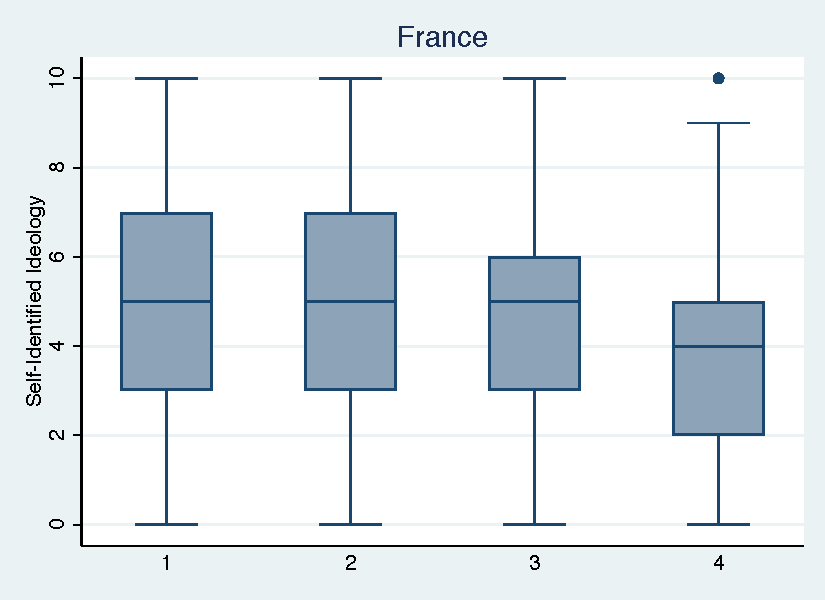
\includegraphics[width=\textwidth]{IdeoBP/France}
		\caption{Self-Placement Ideology}
	\end{subfigure}
	\hfill
	\begin{subfigure}[b]{0.475\textwidth}
		\centering 
		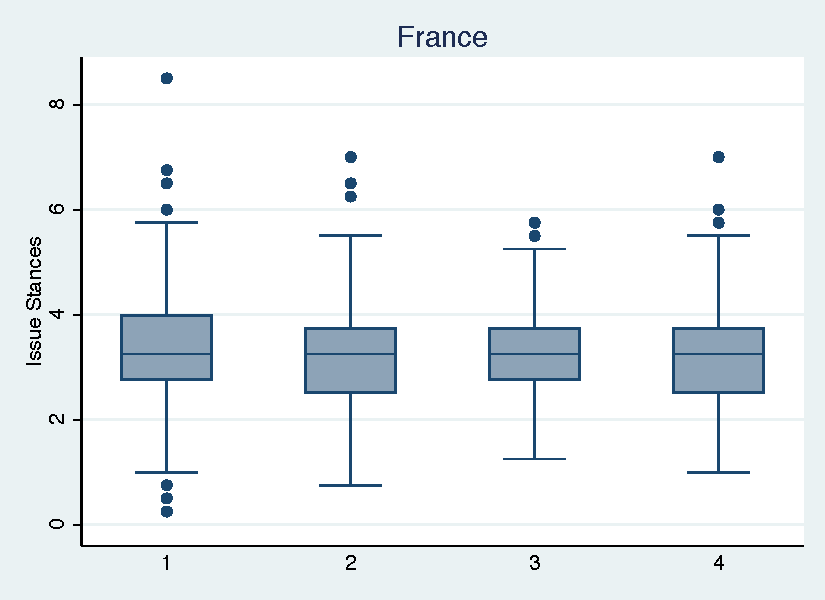
\includegraphics[width=\textwidth]{BoxLib/France}
		\caption{Issue Stances}
	\end{subfigure}
	\caption{France}
	\label{France}
\end{figure}

\begin{figure}[H]
	\centering
	\begin{subfigure}[b]{0.475\textwidth}   
		\centering 
		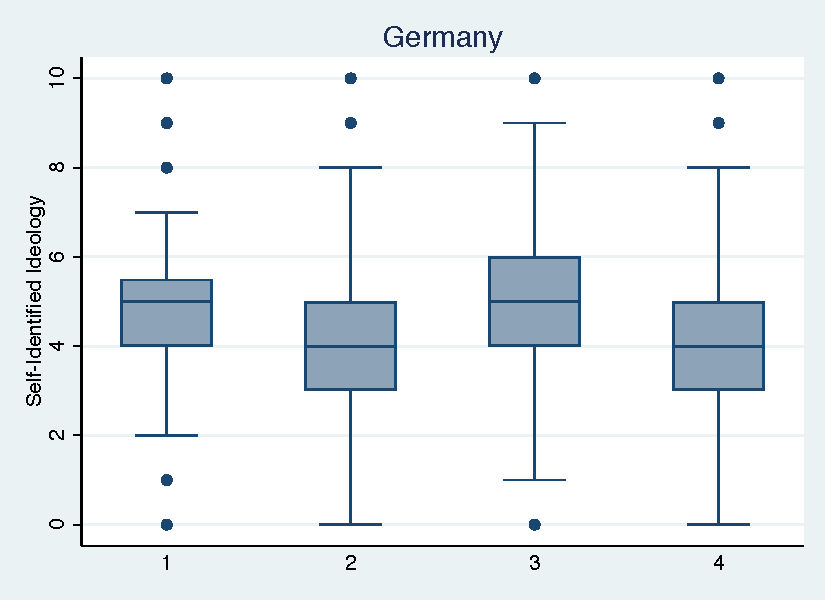
\includegraphics[width=\textwidth]{IdeoBP/Germany}
		\caption{Self-Placement Ideology}
	\end{subfigure}
	\hfill
	\begin{subfigure}[b]{0.475\textwidth}
		\centering 
		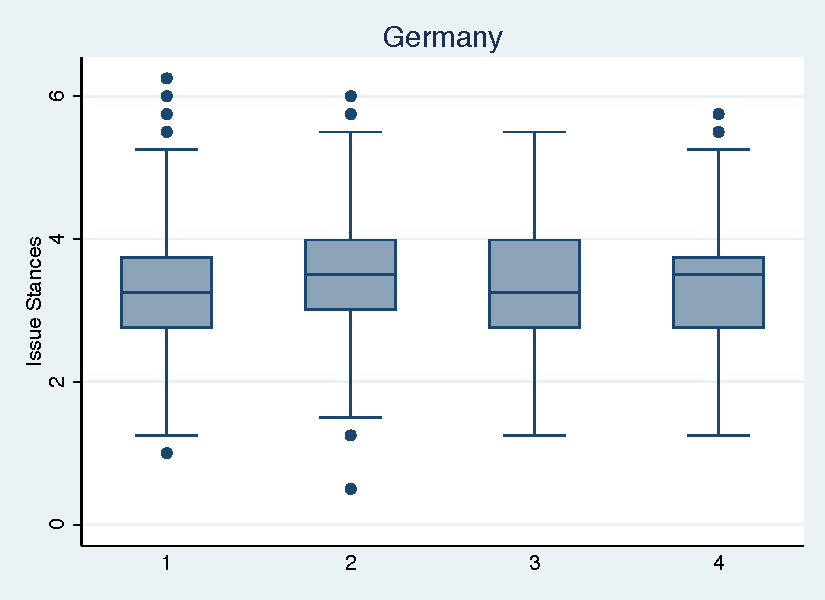
\includegraphics[width=\textwidth]{BoxLib/Germany}
		\caption{Issue Stances}
	\end{subfigure}
	\caption{Germany}
	\label{Germany}
\end{figure}

\begin{figure}[H]
	\centering
	\begin{subfigure}[b]{0.475\textwidth}   
		\centering 
		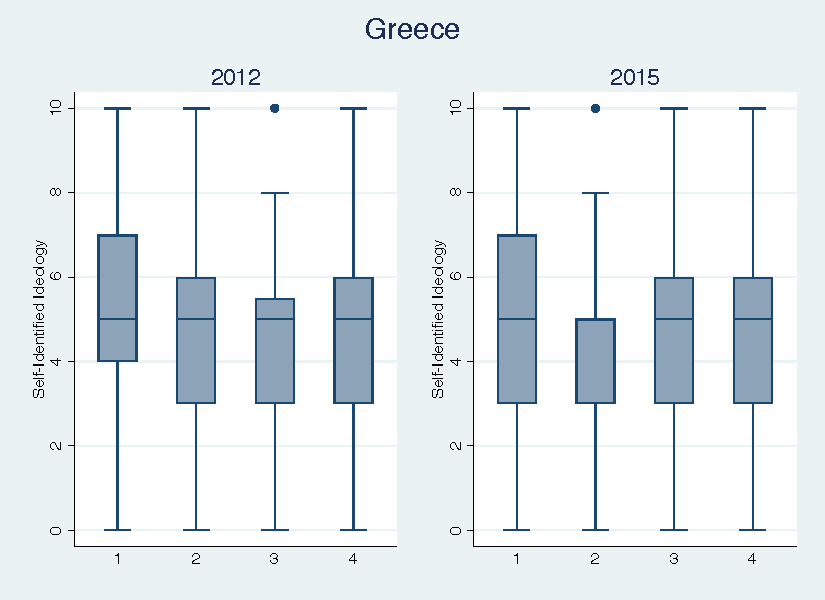
\includegraphics[width=\textwidth]{IdeoBP/Greece}
		\caption{Self-Placement Ideology}
	\end{subfigure}
	\hfill
	\begin{subfigure}[b]{0.475\textwidth}
		\centering 
		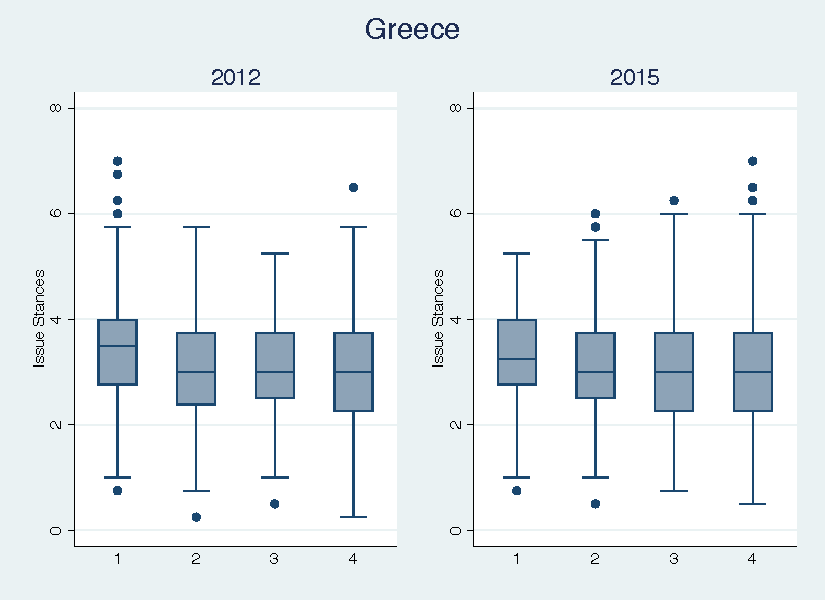
\includegraphics[width=\textwidth]{BoxLib/Greece}
		\caption{Issue Stances}
	\end{subfigure}
	\caption{Greece}
	\label{Greece}
\end{figure}

\begin{figure}[H]
	\centering
	\begin{subfigure}[b]{0.475\textwidth}   
		\centering 
		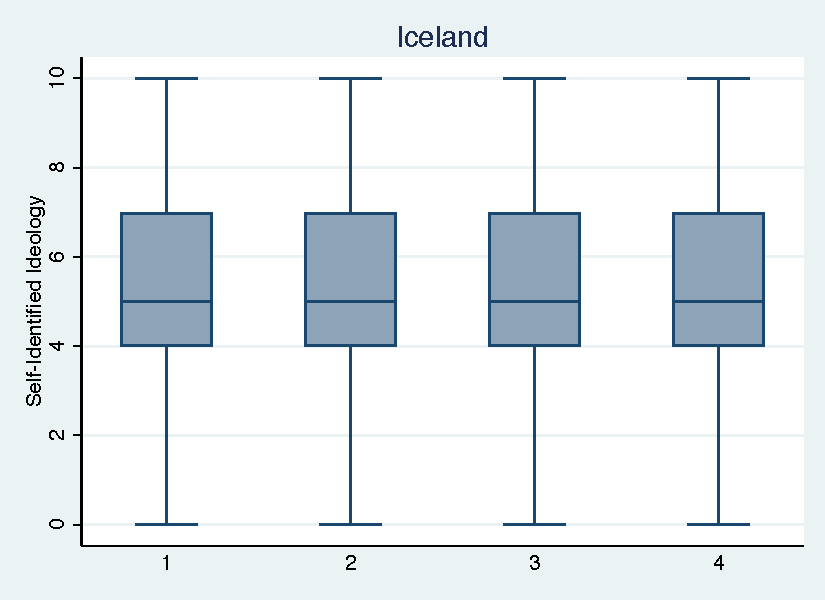
\includegraphics[width=\textwidth]{IdeoBP/Iceland}
		\caption{Self-Placement Ideology}
	\end{subfigure}
	\hfill
	\begin{subfigure}[b]{0.475\textwidth}
		\centering 
		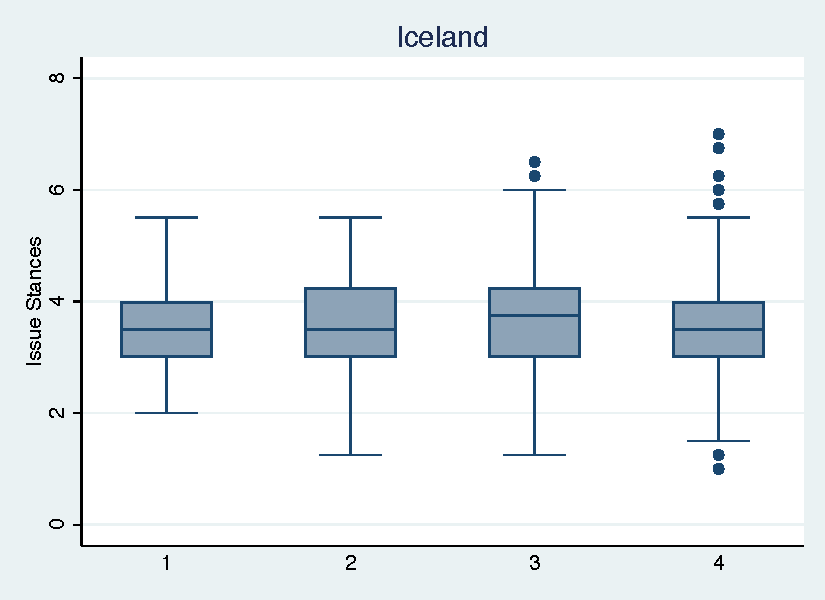
\includegraphics[width=\textwidth]{BoxLib/Iceland}
		\caption{Issue Stances}
	\end{subfigure}
	\caption{Iceland}
	\label{Iceland}
\end{figure}

\begin{figure}[H]
	\centering
	\begin{subfigure}[b]{0.475\textwidth}   
		\centering 
		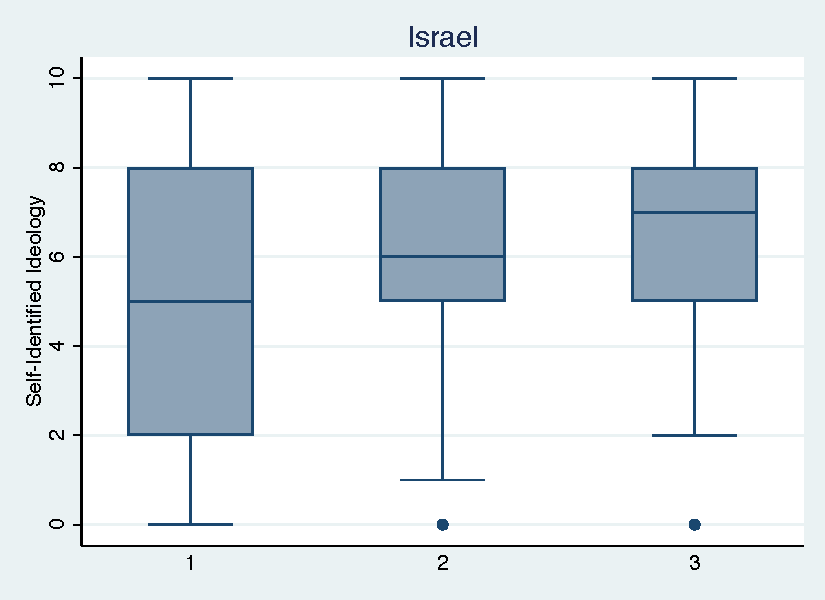
\includegraphics[width=\textwidth]{IdeoBP/Israel}
		\caption{Self-Placement Ideology}
	\end{subfigure}
	\hfill
	\begin{subfigure}[b]{0.475\textwidth}
		\centering 
		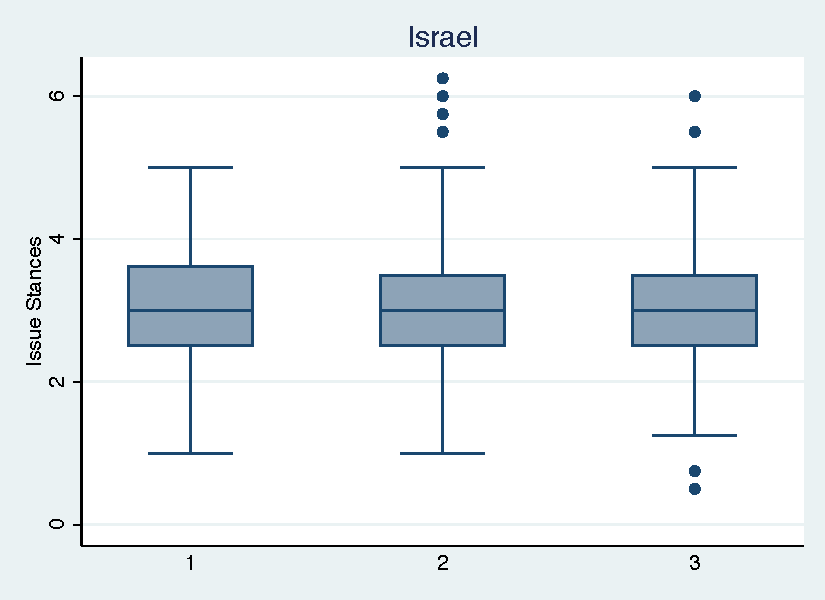
\includegraphics[width=\textwidth]{BoxLib/Israel}
		\caption{Issue Stances}
	\end{subfigure}
	\caption{Israel}
	\label{Israel}
\end{figure}

\begin{figure}[H]
	\centering
	\begin{subfigure}[b]{0.475\textwidth}   
		\centering 
		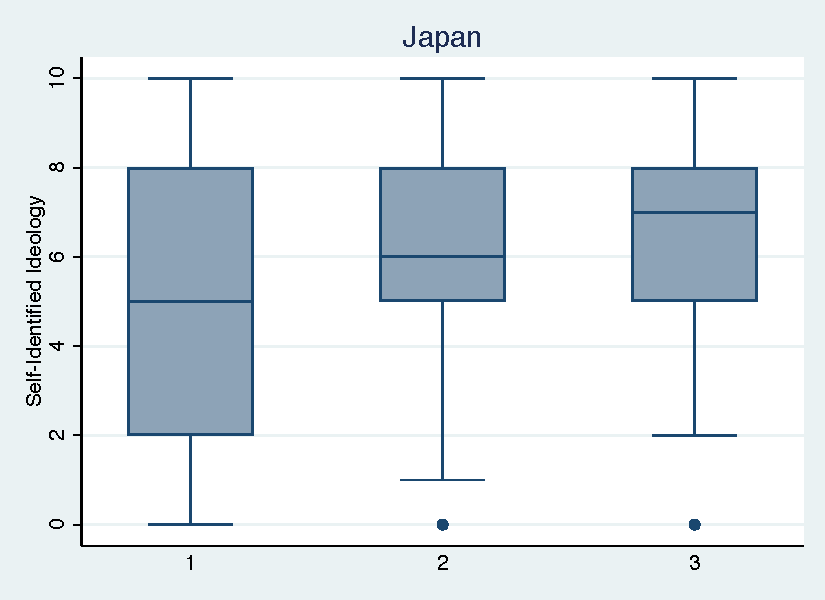
\includegraphics[width=\textwidth]{IdeoBP/Japan}
		\caption{Self-Placement Ideology}
	\end{subfigure}
	\hfill
	\begin{subfigure}[b]{0.475\textwidth}
		\centering 
		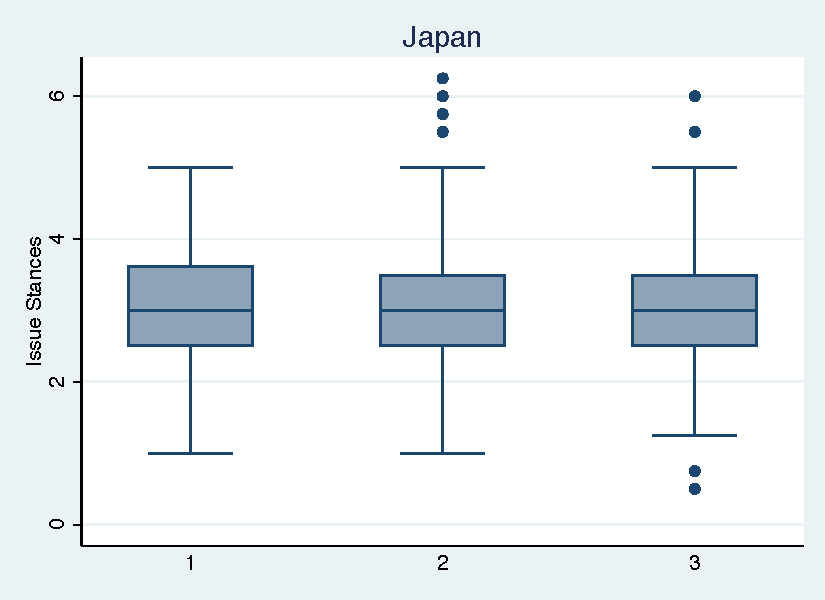
\includegraphics[width=\textwidth]{BoxLib/Japan}
		\caption{Issue Stances}
	\end{subfigure}
	\caption{Japan}
	\label{Japan}
\end{figure}

\begin{figure}[H]
	\centering
	\begin{subfigure}[b]{0.475\textwidth}   
		\centering 
		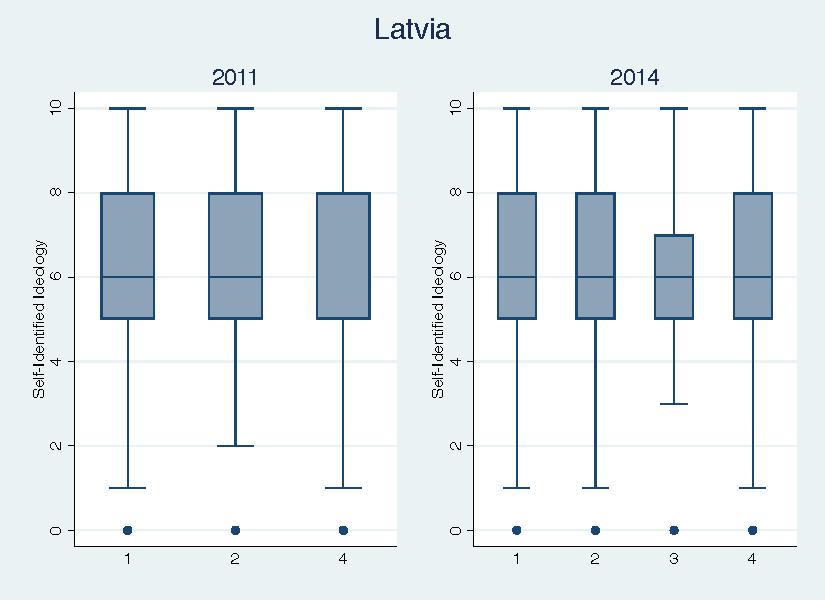
\includegraphics[width=\textwidth]{IdeoBP/Latvia}
		\caption{Self-Placement Ideology}
	\end{subfigure}
	\hfill
	\begin{subfigure}[b]{0.475\textwidth}
		\centering 
		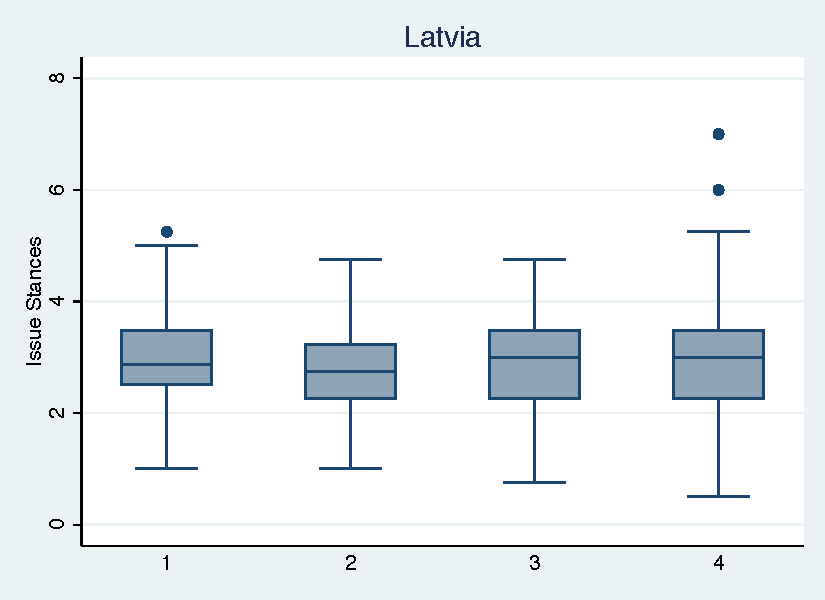
\includegraphics[width=\textwidth]{BoxLib/Latvia}
		\caption{Issue Stances}
	\end{subfigure}
	\caption{Latvia}
	\label{Latvia}
\end{figure}

\begin{figure}[H]
	\centering
	\begin{subfigure}[b]{0.475\textwidth}   
		\centering 
		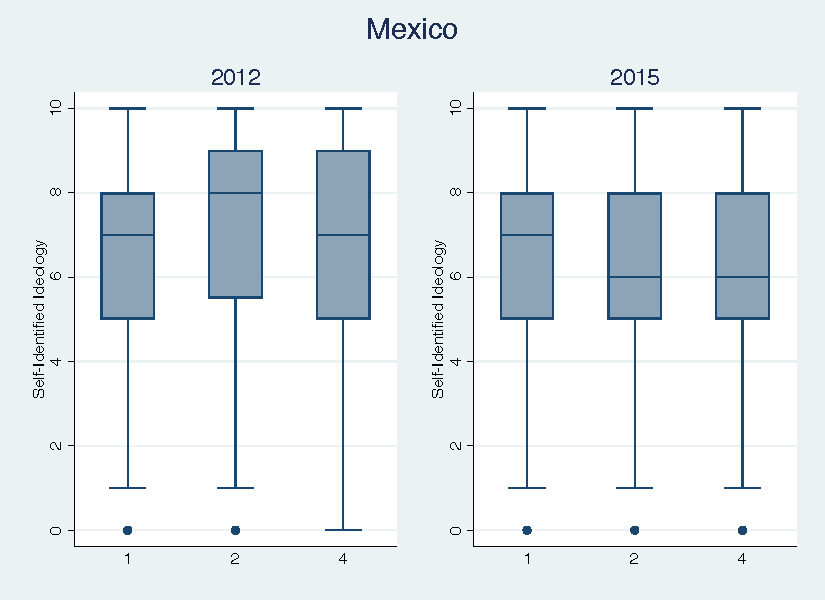
\includegraphics[width=\textwidth]{IdeoBP/Mexico}
		\caption{Self-Placement Ideology}
	\end{subfigure}
	\hfill
	\begin{subfigure}[b]{0.475\textwidth}
		\centering 
		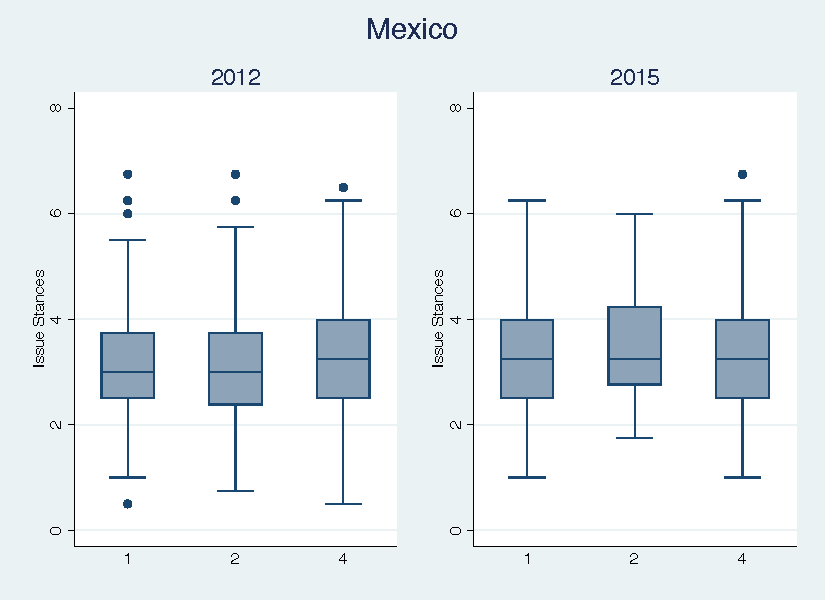
\includegraphics[width=\textwidth]{BoxLib/Mexico}
		\caption{Issue Stances}
	\end{subfigure}
	\caption{Mexico}
	\label{Mexico}
\end{figure}

\begin{figure}[H]
	\centering
	\begin{subfigure}[b]{0.475\textwidth}   
		\centering 
		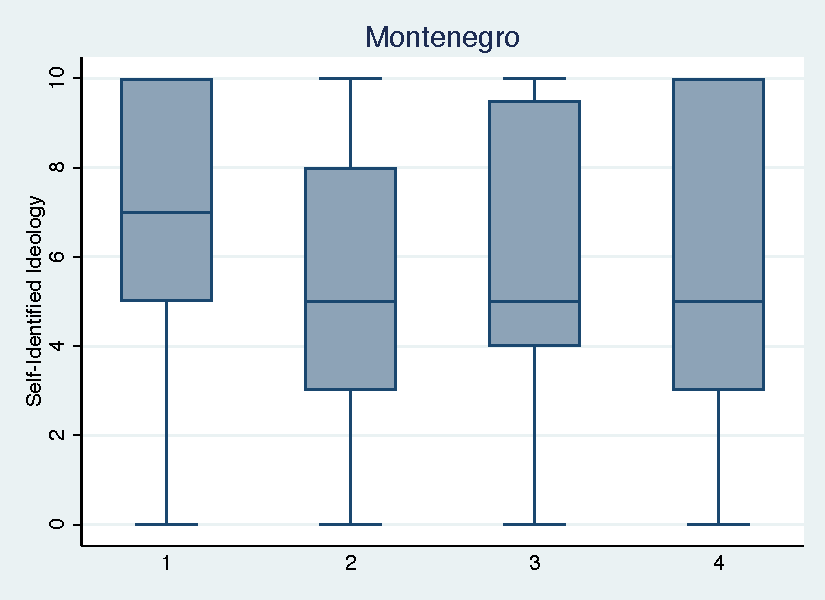
\includegraphics[width=\textwidth]{IdeoBP/Montenegro}
		\caption{Self-Placement Ideology}
	\end{subfigure}
	\hfill
	\begin{subfigure}[b]{0.475\textwidth}
		\centering 
		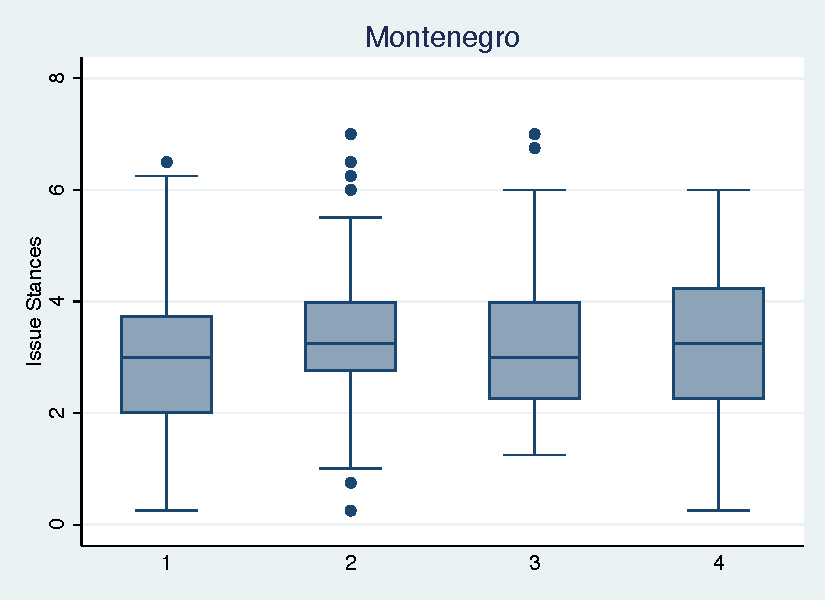
\includegraphics[width=\textwidth]{BoxLib/Montenegro}
		\caption{Issue Stances}
	\end{subfigure}
	\caption{Montenegro}
	\label{Montenegro}
\end{figure}

\begin{figure}[H]
	\centering
	\begin{subfigure}[b]{0.475\textwidth}   
		\centering 
		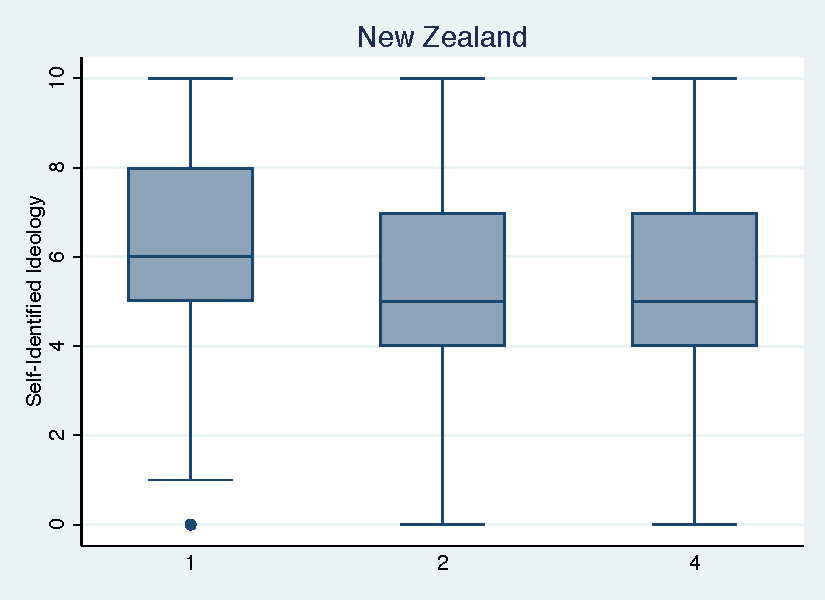
\includegraphics[width=\textwidth]{IdeoBP/NewZealand}
		\caption{Self-Placement Ideology}
	\end{subfigure}
	\hfill
	\begin{subfigure}[b]{0.475\textwidth}
		\centering 
		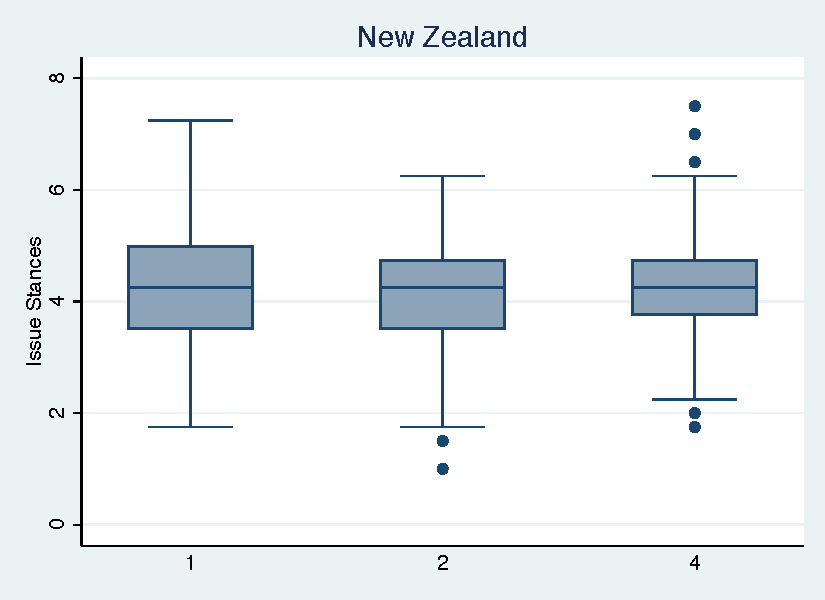
\includegraphics[width=\textwidth]{BoxLib/NZealand}
		\caption{Issue Stances}
	\end{subfigure}
	\caption{New Zealand}
	\label{NewZealand}
\end{figure}

\begin{figure}[H]
	\centering
	\begin{subfigure}[b]{0.475\textwidth}   
		\centering 
		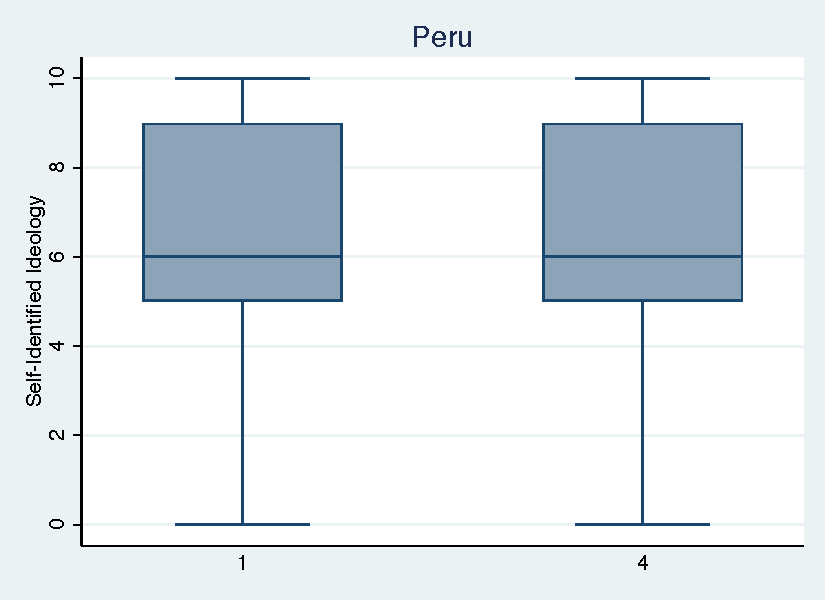
\includegraphics[width=\textwidth]{IdeoBP/Peru}
		\caption{Self-Placement Ideology}
	\end{subfigure}
	\hfill
	\begin{subfigure}[b]{0.475\textwidth}
		\centering 
		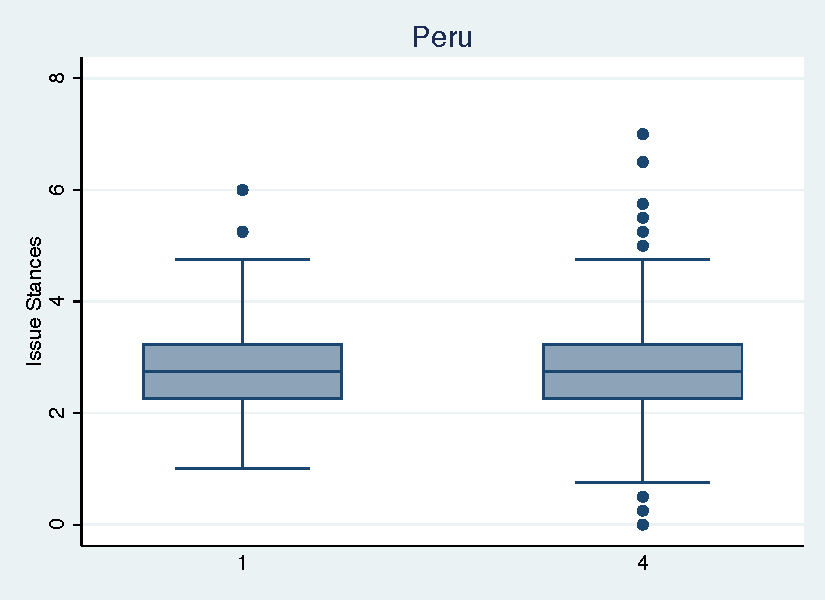
\includegraphics[width=\textwidth]{BoxLib/Peru}
		\caption{Issue Stances}
	\end{subfigure}
	\caption{Peru}
	\label{Peru}
\end{figure}

\begin{figure}[H]
	\centering
	\begin{subfigure}[b]{0.475\textwidth}   
		\centering 
		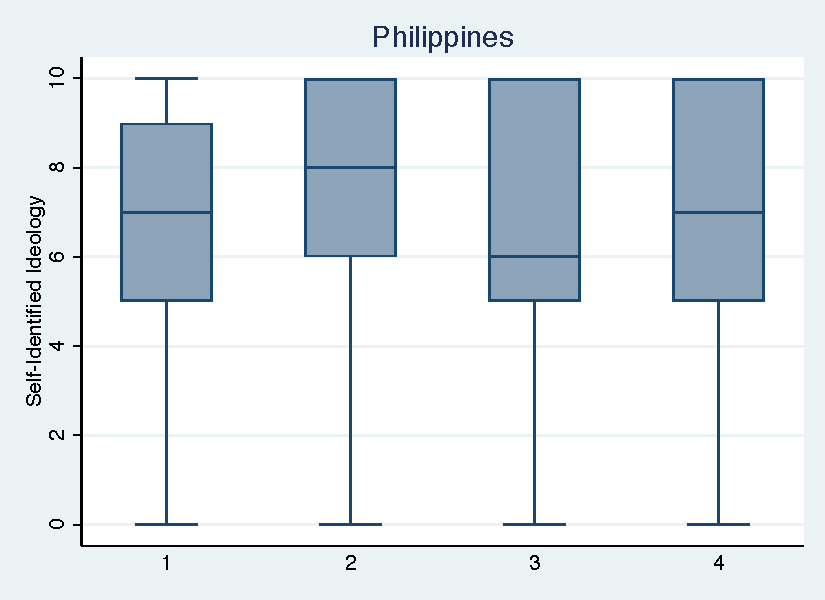
\includegraphics[width=\textwidth]{IdeoBP/Philippines}
		\caption{Self-Placement Ideology}
	\end{subfigure}
	\hfill
	\begin{subfigure}[b]{0.475\textwidth}
		\centering 
		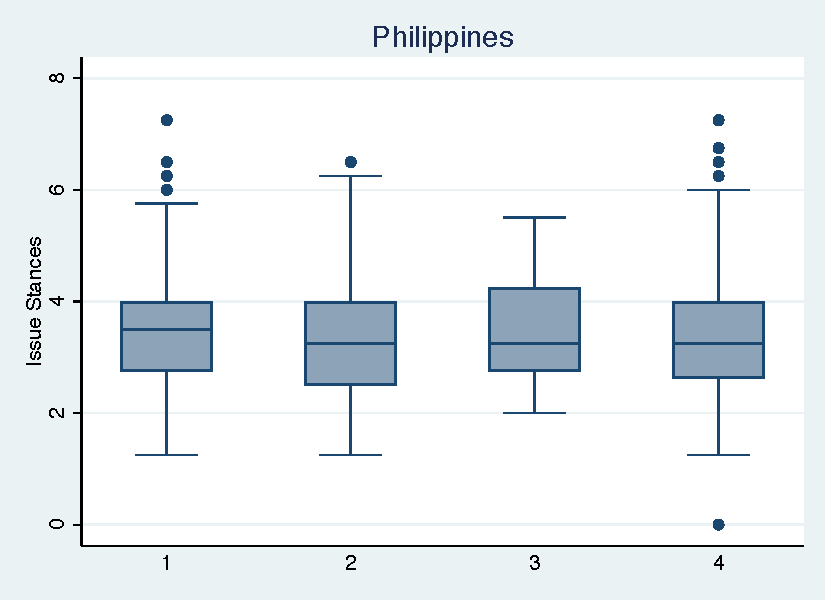
\includegraphics[width=\textwidth]{BoxLib/Philipines}
		\caption{Issue Stances}
	\end{subfigure}
	\caption{Philippines}
	\label{Philippines}
\end{figure}

\begin{figure}[H]
	\centering
	\begin{subfigure}[b]{0.475\textwidth}   
		\centering 
		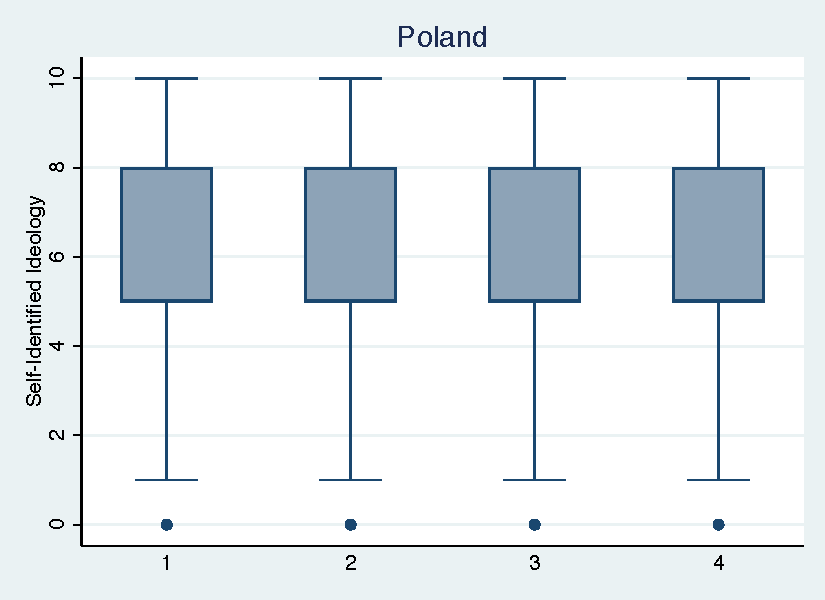
\includegraphics[width=\textwidth]{IdeoBP/Poland}
		\caption{Self-Placement Ideology}
	\end{subfigure}
	\hfill
	\begin{subfigure}[b]{0.475\textwidth}
		\centering 
		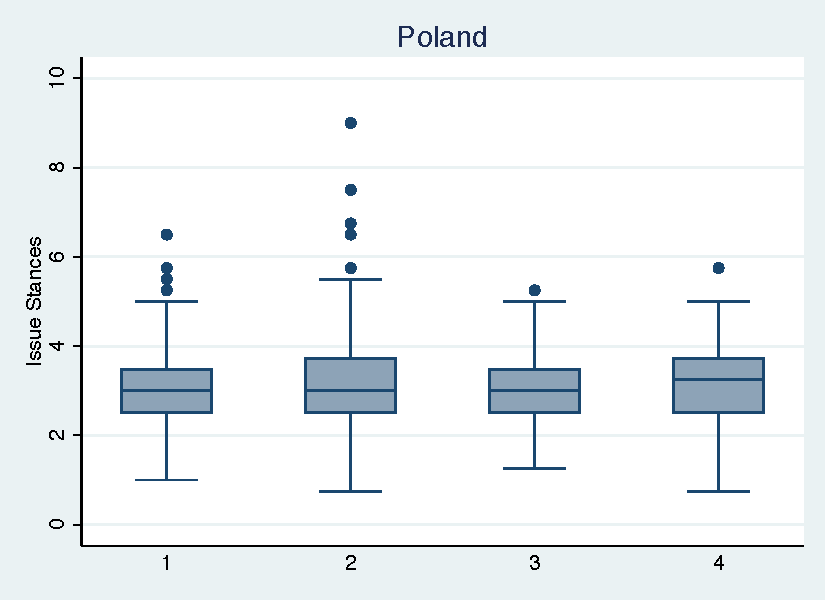
\includegraphics[width=\textwidth]{BoxLib/Poland}
		\caption{Issue Stances}
	\end{subfigure}
	\caption{Poland}
	\label{Poland}
\end{figure}

\begin{figure}[H]
	\centering
	\begin{subfigure}[b]{0.475\textwidth}   
		\centering 
		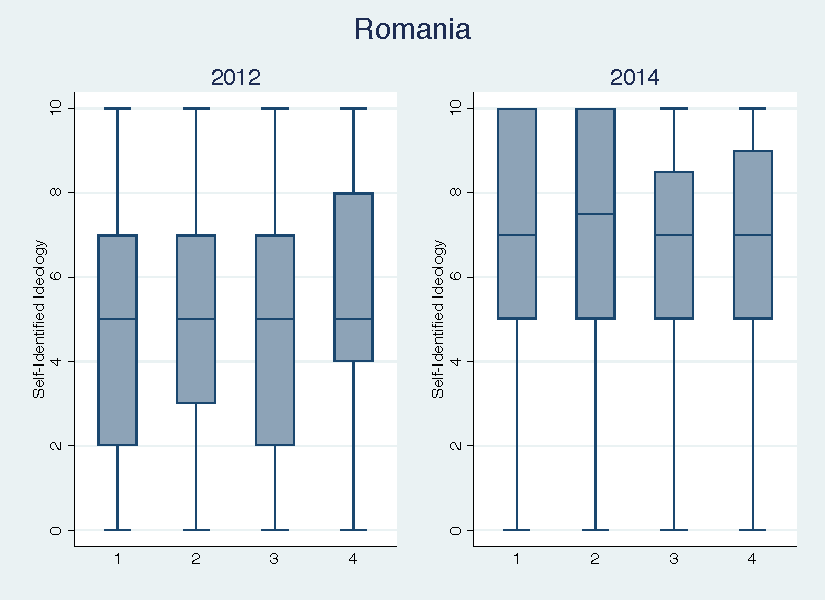
\includegraphics[width=\textwidth]{IdeoBP/Romania}
		\caption{Self-Placement Ideology}
	\end{subfigure}
	\hfill
	\begin{subfigure}[b]{0.475\textwidth}
		\centering 
		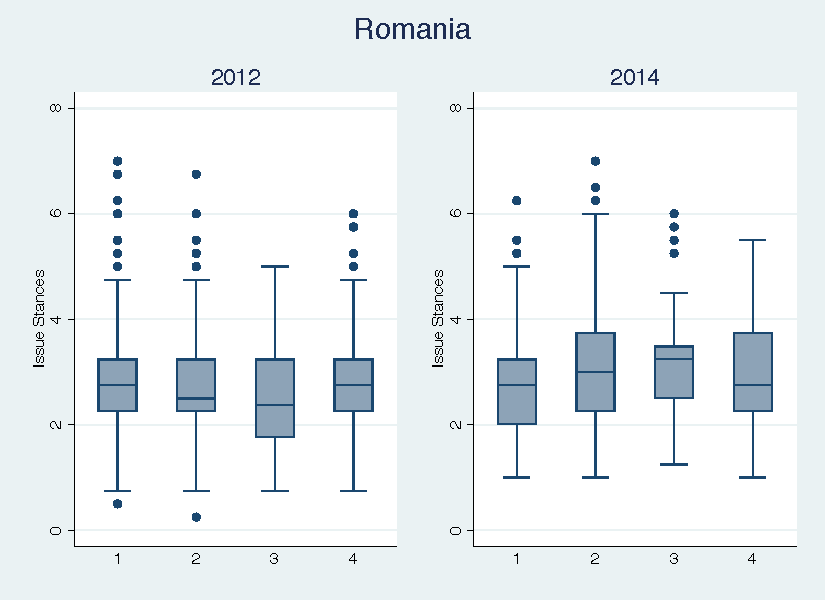
\includegraphics[width=\textwidth]{BoxLib/Romania}
		\caption{Issue Stances}
	\end{subfigure}
	\caption{Romania}
	\label{Romania}
\end{figure}

\begin{figure}[H]
		\centering 
		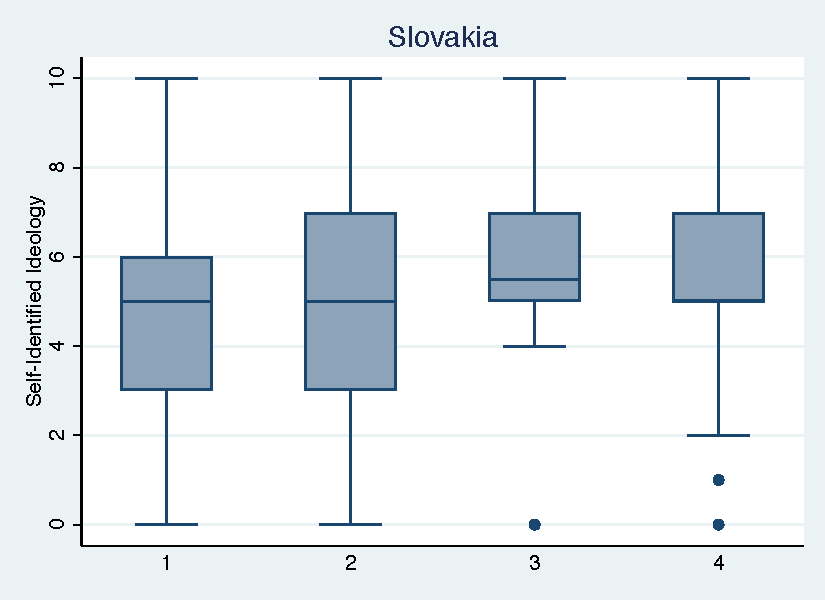
\includegraphics[width=\textwidth]{IdeoBP/Slovakia}
	\caption{Slovakia - Self-Placement Ideology}
	\label{Slovakia}
\end{figure}

\begin{figure}[H]
	\centering
	\begin{subfigure}[b]{0.475\textwidth}   
		\centering 
		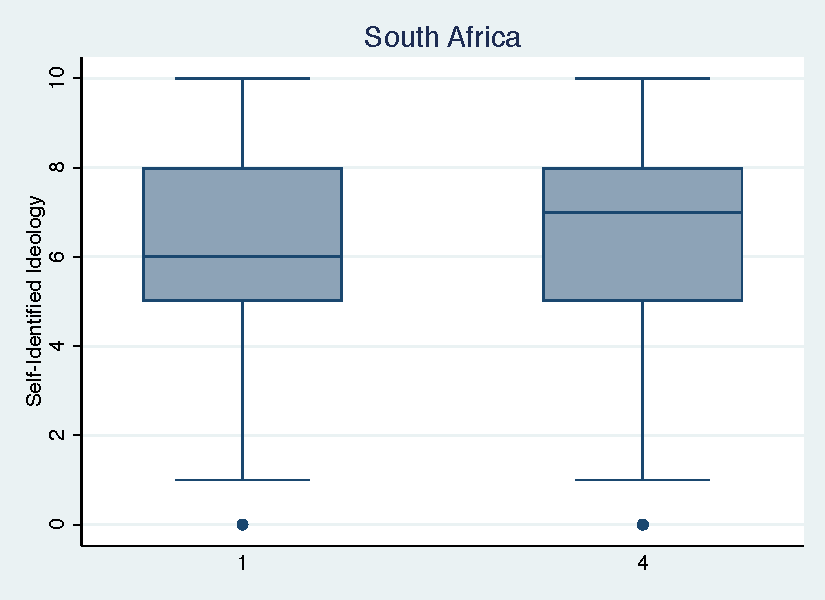
\includegraphics[width=\textwidth]{IdeoBP/SouthAfrica}
		\caption{Self-Placement Ideology}
	\end{subfigure}
	\hfill
	\begin{subfigure}[b]{0.475\textwidth}
		\centering 
		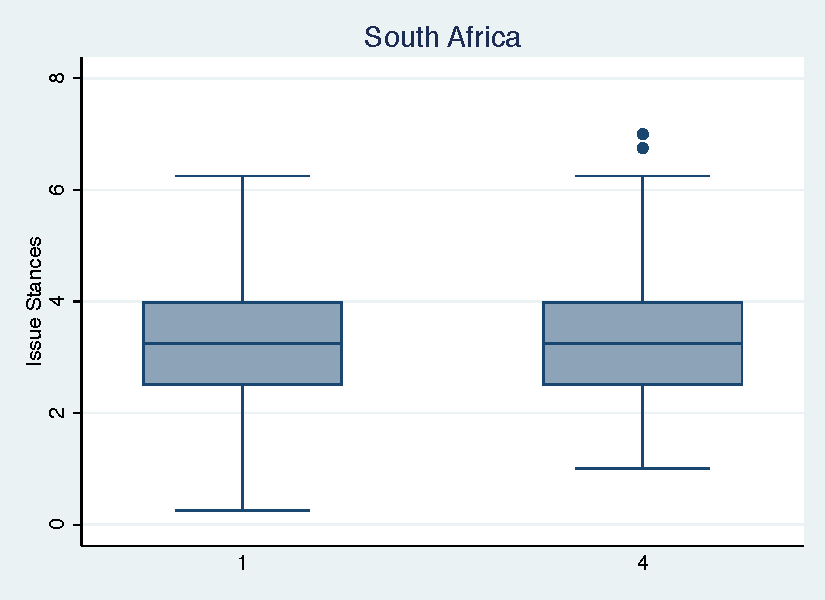
\includegraphics[width=\textwidth]{BoxLib/SAfrica}
		\caption{Issue Stances}
	\end{subfigure}
	\caption{South Africa}
	\label{SouthAfrica}
\end{figure}

\begin{figure}[H]
	\centering
	\begin{subfigure}[b]{0.475\textwidth}   
		\centering 
		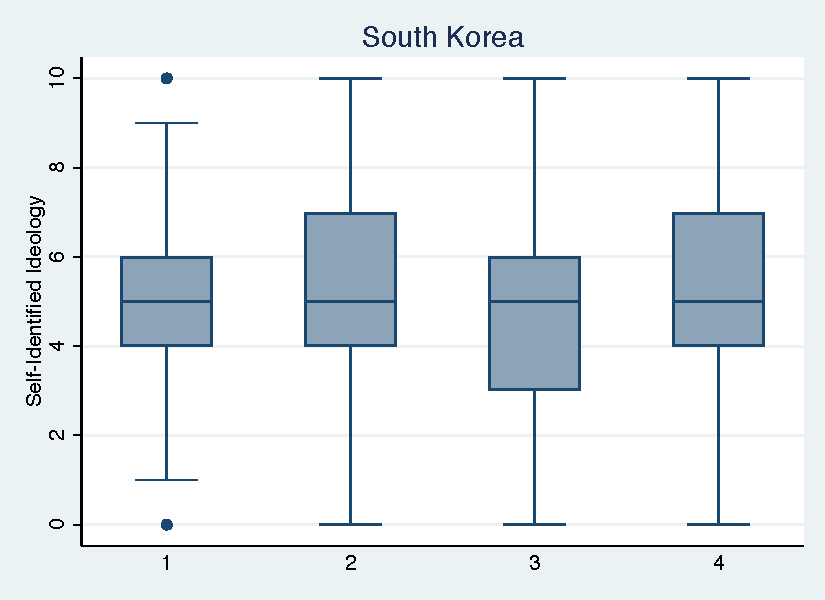
\includegraphics[width=\textwidth]{IdeoBP/SouthKorea}
		\caption{Self-Placement Ideology}
	\end{subfigure}
	\hfill
	\begin{subfigure}[b]{0.475\textwidth}
		\centering 
		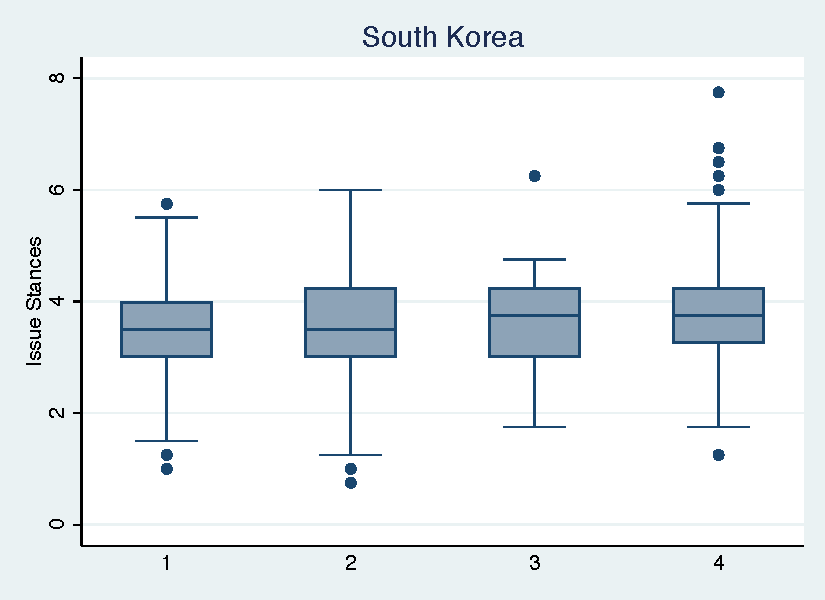
\includegraphics[width=\textwidth]{BoxLib/SKorea}
		\caption{Issue Stances}
	\end{subfigure}
	\caption{South Korea}
	\label{SouthKorea}
\end{figure}

\begin{figure}[H]
	\centering
	\begin{subfigure}[b]{0.475\textwidth}   
		\centering 
		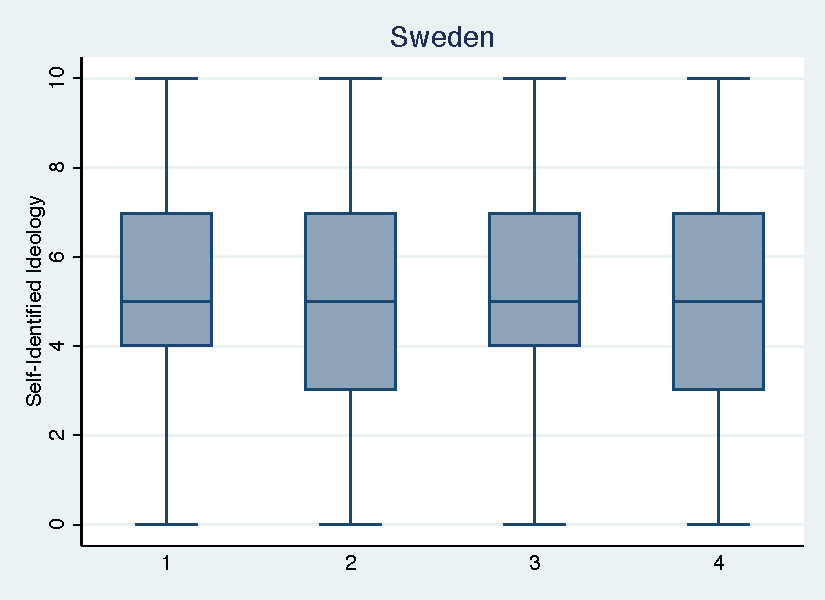
\includegraphics[width=\textwidth]{IdeoBP/Sweden}
		\caption{Self-Placement Ideology}
	\end{subfigure}
	\hfill
	\begin{subfigure}[b]{0.475\textwidth}
		\centering 
		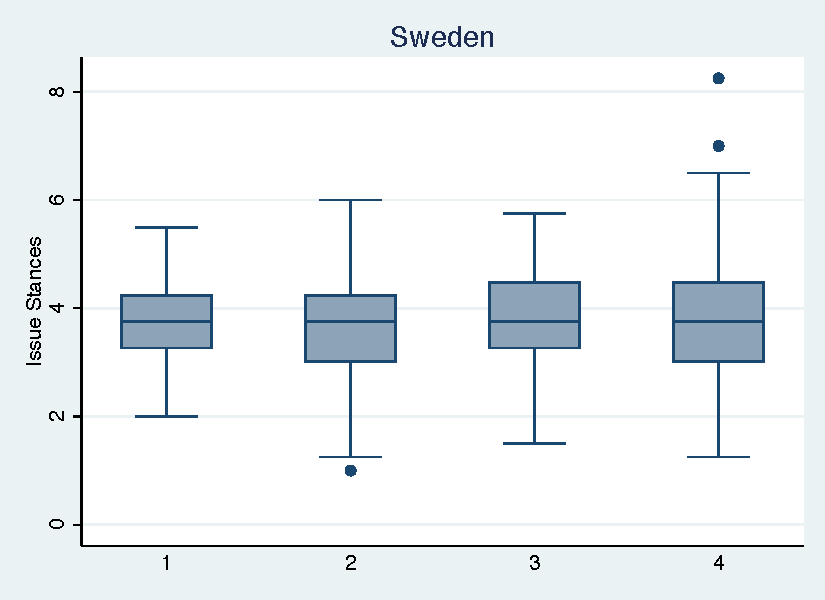
\includegraphics[width=\textwidth]{BoxLib/Sweden}
		\caption{Issue Stances}
	\end{subfigure}
	\caption{Sweden}
	\label{Sweden}
\end{figure}

\begin{figure}[H]
	\centering
	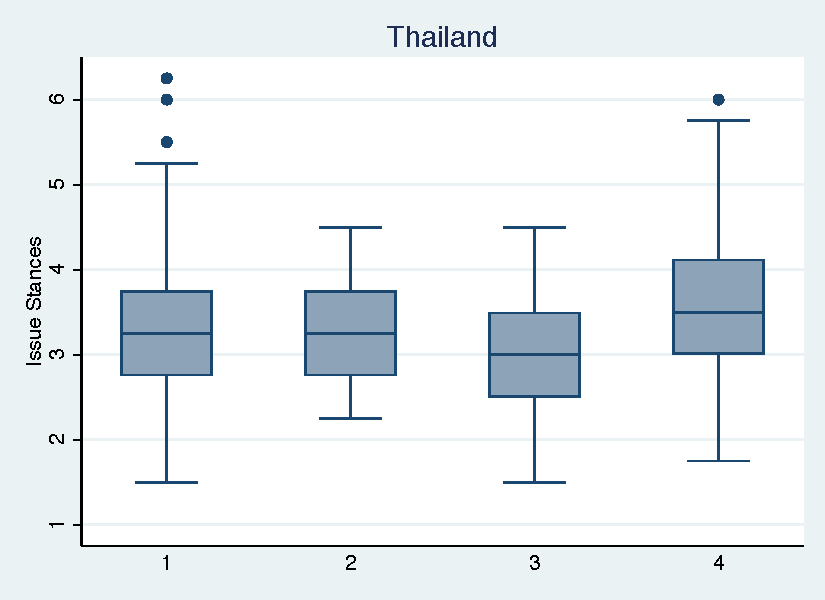
\includegraphics[width=\textwidth]{BoxLib/Thailand}
	\caption{Thailand - Issue Stances}
	\label{Thailand}
\end{figure}

\begin{figure}[H]
	\centering
	\begin{subfigure}[b]{0.475\textwidth}   
		\centering 
		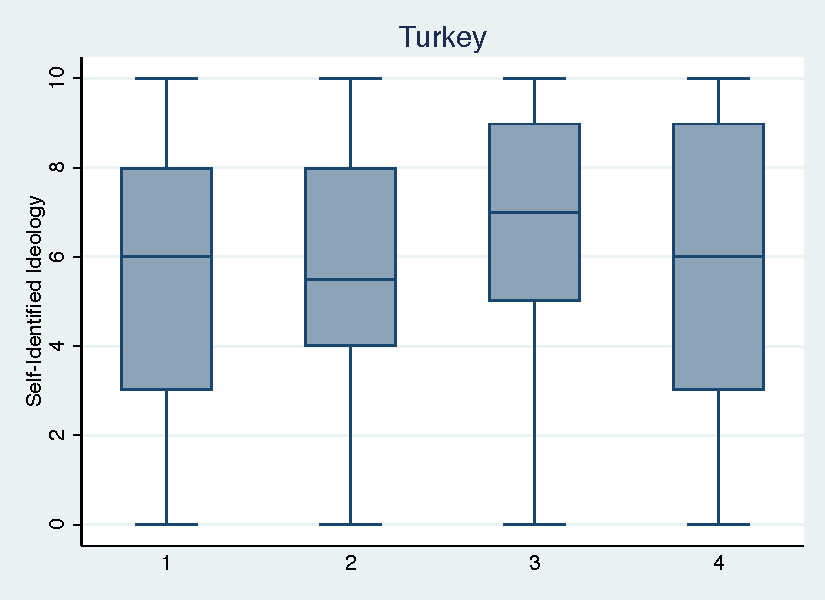
\includegraphics[width=\textwidth]{IdeoBP/Turkey}
		\caption{Self-Placement Ideology}
	\end{subfigure}
	\hfill
	\begin{subfigure}[b]{0.475\textwidth}
		\centering 
		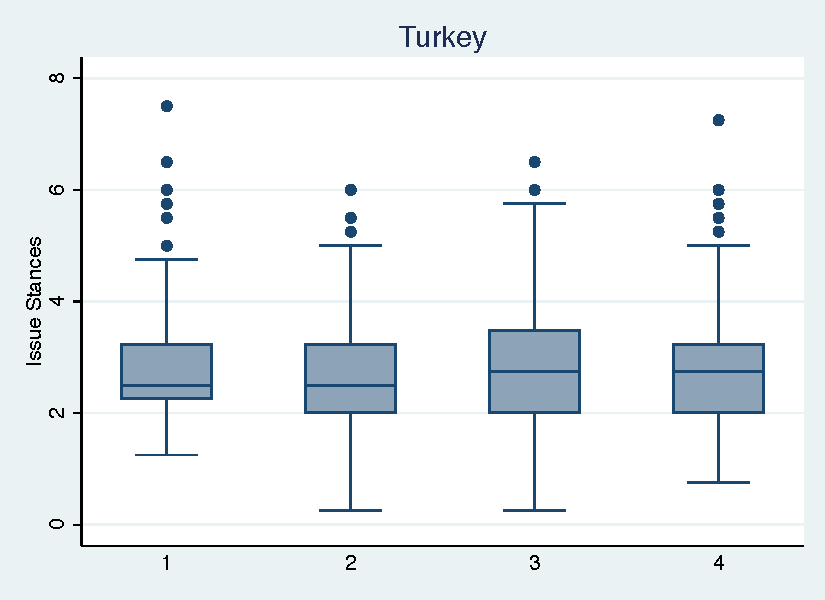
\includegraphics[width=\textwidth]{BoxLib/Turkey}
		\caption{Issue Stances}
	\end{subfigure}
	\caption{Turkey}
	\label{Turkey}
\end{figure}

\end{document}